\documentclass[aspectratio=169,10pt]{beamer}
% Message & body slide style. Compile with xelatex.
\usepackage{xeCJK}
\setCJKmainfont[BoldFont={Hiragino Sans W6}]{Hiragino Sans W3}
\setCJKsansfont[BoldFont={Hiragino Sans W6}]{Hiragino Sans W3}
\setmainfont{Helvetica Neue}
\setsansfont{Helvetica Neue}
% circled digits and arrows must come from the Japanese font
\xeCJKDeclareCharClass{FullLeft}{"2460->"2473}
\xeCJKDeclareCharClass{CJK}{"2192, "2190, "2460->"2473}
\usepackage{graphicx,booktabs,tabularx,array,colortbl,xcolor,tikz,multirow}
\usetikzlibrary{arrows.meta,positioning,shapes.misc}

\definecolor{ink}{HTML}{1A202C}
\definecolor{muted}{HTML}{6B6B6B}
\definecolor{accent}{HTML}{2B6CB0}
\definecolor{accent2}{HTML}{C05621}
\definecolor{good}{HTML}{2F855A}
\definecolor{bad}{HTML}{C53030}
\definecolor{soft}{HTML}{F2F5F9}
\definecolor{rule}{HTML}{D5DCE4}

\setbeamertemplate{navigation symbols}{}
\setbeamercolor{normal text}{fg=ink}
\setbeamerfont{normal text}{size=\small}
\setbeamercolor{structure}{fg=accent}
\setbeamertemplate{itemize item}{\color{accent}\raisebox{0.15ex}{\scriptsize$\blacksquare$}}
\setbeamertemplate{itemize subitem}{\color{muted}--}
\setlength{\leftmargini}{1.1em}

% --- frame title = section tag (small) + message (1-2 sentences) ---
\newcommand{\slidetag}{}
\newcommand{\settag}[1]{\renewcommand{\slidetag}{#1}}
\setbeamertemplate{frametitle}{%
  \vspace{0.35cm}%
  \begin{minipage}{\textwidth}
    {\color{accent}\scriptsize\bfseries\slidetag}\par\vspace{0.12cm}
    {\color{ink}\large\bfseries\insertframetitle\par}
    \vspace{0.18cm}{\color{rule}\rule{\textwidth}{0.8pt}}
  \end{minipage}}
\setbeamertemplate{footline}{%
  \leavevmode\hbox to\paperwidth{\hspace{0.45cm}{\color{muted}\tiny ETT Oil-Temperature Forecasting PoC}\hfill
  {\color{muted}\tiny\insertframenumber}\hspace{0.45cm}}\vspace{0.22cm}}

\newcommand{\source}[1]{\vfill{\color{muted}\tiny #1}}
\newcommand{\hl}[1]{{\color{accent}\bfseries #1}}
\newcommand{\hlb}[1]{{\color{bad}\bfseries #1}}
\newcommand{\hlg}[1]{{\color{good}\bfseries #1}}
\newcommand{\fig}[2][]{\includegraphics[#1]{../outputs/figures/#2.png}}
\newcommand{\softbox}[2]{\begin{beamercolorbox}[sep=6pt,rounded=false]{soft}#2\end{beamercolorbox}}
\setbeamercolor{soft}{bg=soft,fg=ink}
\newcommand{\kpi}[3]{% value, label, color
  \begin{minipage}[t]{0.23\textwidth}\centering
    {\color{#3}\fontsize{20}{22}\selectfont\bfseries #1}\par\vspace{0.1cm}
    {\scriptsize\color{muted}#2}
  \end{minipage}}

\graphicspath{{../outputs/figures/}}

\begin{document}

% ------------------------------------------------------------------ title
{\setbeamertemplate{footline}{}
\begin{frame}[plain]
  \vspace{1.2cm}
  {\color{accent}\small\bfseries Proof-of-Concept Report}\par\vspace{0.3cm}
  {\color{ink}\LARGE\bfseries Forecasting Transformer Oil Temperature\\[0.15cm]24 Hours Ahead for Preventive Maintenance}\par\vspace{0.4cm}
  {\color{muted}\normalsize A study on the public ETT benchmark dataset (ETTh1 / ETTh2)}\par
  \vfill
  {\color{rule}\rule{\textwidth}{0.8pt}}\par\vspace{0.15cm}
  {\small Pyii Phyo Maung}\hfill{\small\color{muted}November 2026}
  \vspace{0.6cm}
\end{frame}}

% ------------------------------------------------------------------ 1 summary
\settag{Executive summary}
\begin{frame}{Forecasts flag 80\% of overheating onsets about 23 h ahead but improve accuracy by only 5--9\%; deployment needs ambient data}
  \kpi{−9.1\%}{24 h error vs.\\persistence (ETTh1)}{accent}\hfill
  \kpi{80\%}{Onsets warned early\\(ETTh2, 10 false h/month)}{good}\hfill
  \kpi{$\sim$23 h}{Median warning\\lead time}{accent2}\hfill
  \kpi{0 h}{Lead time of today's\\threshold alarm}{bad}
  \vspace{0.2cm}
  \begin{columns}[T]
    \begin{column}{0.49\textwidth}
      \softbox{}{\scriptsize\textbf{Findings}
      \begin{itemize}\setlength{\itemsep}{1pt}
        \item Strong inertia limits the 24 h gain to 5--9\%, but \hl{3--6 h ahead error falls 13--53\%}
        \item Best on ETTh1: physics features + linear model (ETTh2: ensemble, narrowly). GBM, LSTM etc. did not beat it
        \item The value is \emph{warning lead time}, not accuracy; the next-day load plan is key
        \item Raw intervals under-cover (75--84\%); conformal calibration gives 90\%
      \end{itemize}}
    \end{column}
    \begin{column}{0.49\textwidth}
      \softbox{}{\scriptsize\textbf{Recommendations}
      \begin{itemize}\setlength{\itemsep}{1pt}
        \item First, \hl{add ambient temperature} (likely driver of the daily cycle; needed for fault detection)
        \item Share real alarm levels and fault history; validate alerts in a \hl{3-month shadow run}
        \item The data show stuck sensors and fill artefacts: \hl{data-quality monitoring} can start now
      \end{itemize}}
    \end{column}
  \end{columns}
  \source{Evaluation: Jul 2017 -- Jun 2018, 12 monthly rolling folds. Warning rates rest on 15 onsets; the 4 °C margin was read off the evaluation year (exploratory).}
\end{frame}

% ------------------------------------------------------------------ 2 scope
\settag{Question and assumptions}
\begin{frame}{The question is ``can we warn of overheating 24 h ahead?''; we compare forecasts with (C) and without (B) the next-day load plan}
  \begin{columns}[T]
    \begin{column}{0.56\textwidth}
      \centering
      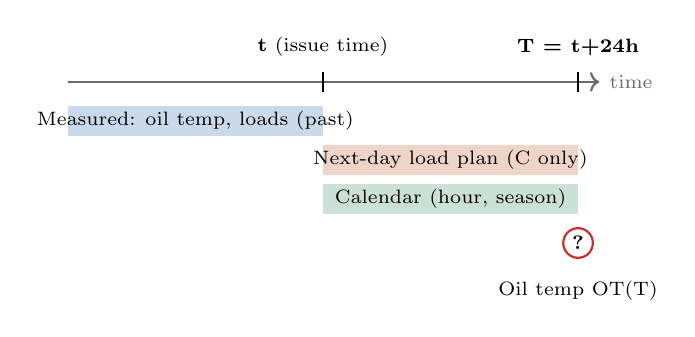
\begin{tikzpicture}[x=0.54cm,y=0.62cm,font=\scriptsize]
        \draw[->,thick,muted] (0,0) -- (12.5,0) node[right]{time};
        \draw[thick] (6,-0.2) -- (6,0.2) node[above=2pt]{\textbf{t} (issue time)};
        \draw[thick] (12,-0.2) -- (12,0.2) node[above=2pt]{\textbf{T = t+24h}};
        \fill[accent!25] (0,-1.1) rectangle (6,-0.5);
        \node at (3,-0.8) {Measured: oil temp, loads (past)};
        \fill[accent2!25] (6,-1.9) rectangle (12,-1.3);
        \node at (9,-1.6) {Next-day load plan (C only)};
        \fill[good!25] (6,-2.7) rectangle (12,-2.1);
        \node at (9,-2.4) {Calendar (hour, season)};
        \node[draw=bad,thick,circle,inner sep=1.5pt,fill=white] at (12,-3.3) {\textbf{?}};
        \node[below=3pt] at (12,-3.7) {Oil temp OT(T)};
      \end{tikzpicture}
    \end{column}
    \begin{column}{0.42\textwidth}
      \footnotesize
      \begin{itemize}\setlength{\itemsep}{3pt}
        \item \textbf{Target}: oil temperature 24 h ahead, the lead time maintenance needs (load shifting, inspection)
        \item \textbf{B (strict)}: only measurements up to t
        \item \textbf{C (plan)}: the ``features at t=T'' the brief allows, read as the \hl{next-day load plan}. Sensitivity to plan error tested (p.14)
        \item \textbf{Value}: accuracy (MAE), plus \hl{how many hours ahead and at how many false alarms} overheating is flagged
        \item No real alarm level was given, so the \hlb{95th percentile of development-period OT} is the proxy alarm
      \end{itemize}
    \end{column}
  \end{columns}
  \source{OT: oil temperature. ETTm1/m2 are the same transformers at 15 min (on-the-hour values equal ETTh1/h2); hourly data assumed enough for 24 h decisions.}
\end{frame}

% ------------------------------------------------------------------ 3 data quality
\settag{EDA ① Data quality}
\begin{frame}{The data freeze on every 31st and have sensors stuck for up to 43 days; left in, these would distort the evaluation itself}
  \begin{columns}[T]
    \begin{column}{0.62\textwidth}
      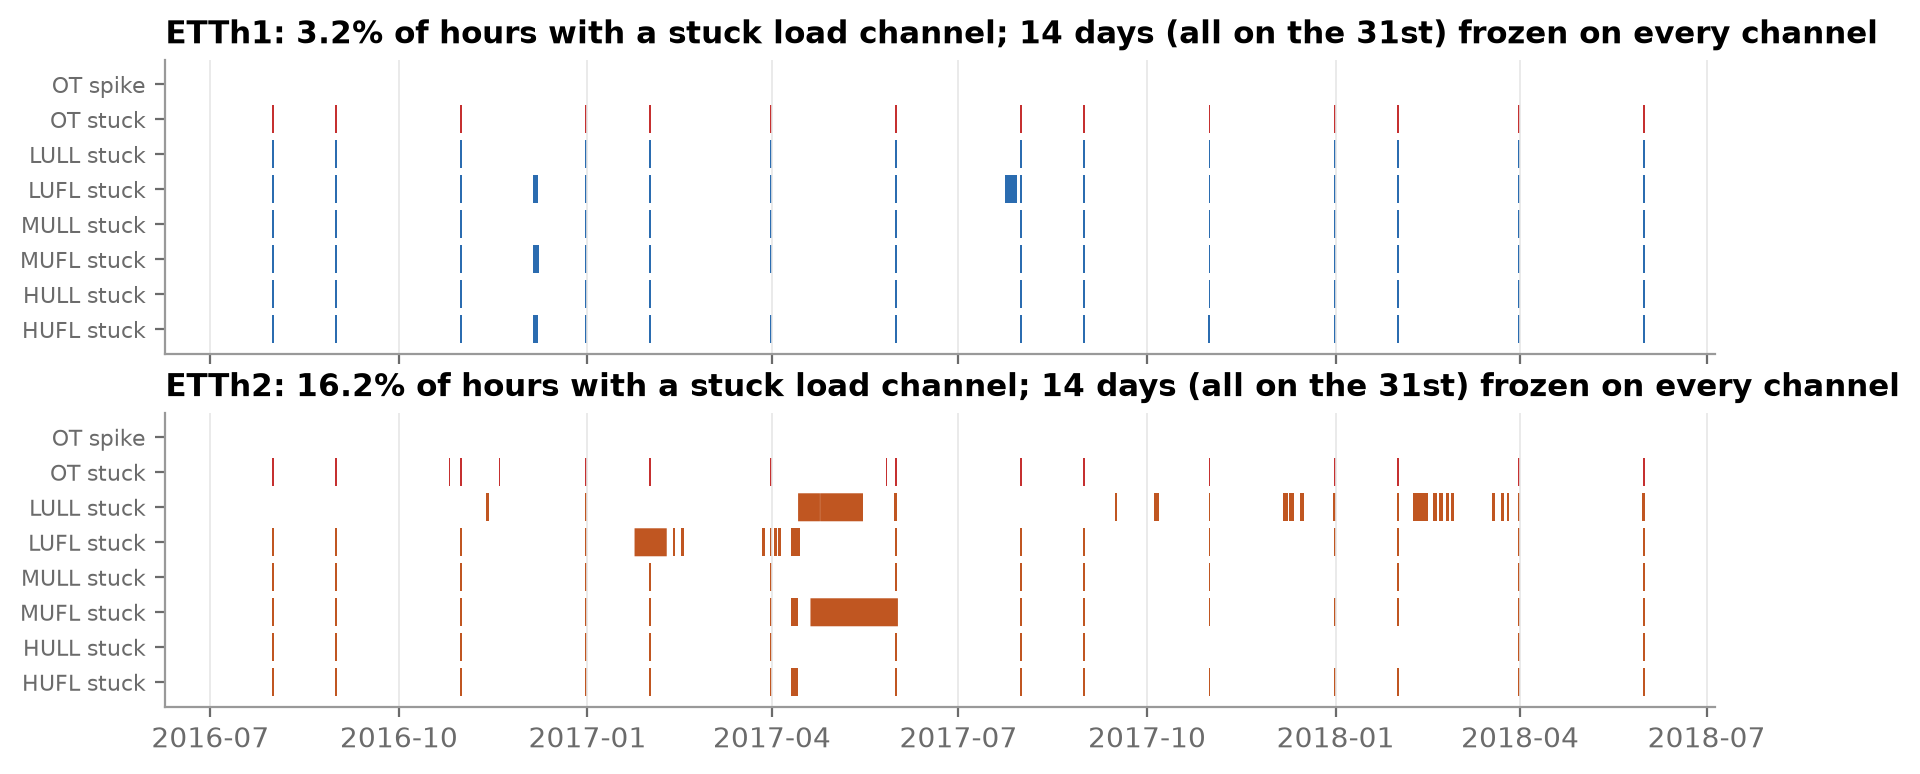
\includegraphics[width=\textwidth]{eda_data_quality}
    \end{column}
    \begin{column}{0.36\textwidth}
      \scriptsize
      \begin{itemize}\setlength{\itemsep}{2pt}
        \item \textbf{31st-day freeze}: \hl{every 31st} is constant on all 7 channels for 24 h, a gap-filling artefact (14 days per transformer)
        \item \textbf{Stuck}: ETTh2 MUFL constant for \hl{1,025 h (43 days)}; stuck share 3.2\% / 16.2\%
        \item \textbf{Spikes}: −20 °C → +23 °C within 1 h (ETTh2)
        \item \textbf{Balance}: assuming high = middle + low (from the column names), it holds on ETTh1 (r=0.99), not ETTh2 (r=0.48)
      \end{itemize}
      \vspace{0.1cm}
      \softbox{}{\scriptsize\textbf{Handling}: invalid targets are not trained on or scored. A stuck input sensor switches the forecast to persistence (past data only, as in operation)}
    \end{column}
  \end{columns}
  \source{Stuck: same value for $\geq$24 h (zero reactive load excluded). Spike: $\geq$6 °C deviation from the centred 5 h median.}
\end{frame}

% ------------------------------------------------------------------ 4 drivers
\settag{EDA ② What drives oil temperature}
\begin{frame}{Oil temperature peaks at 15--16h but load at 0h and 21h: the daily cycle is most likely driven by unmeasured ambient temperature}
  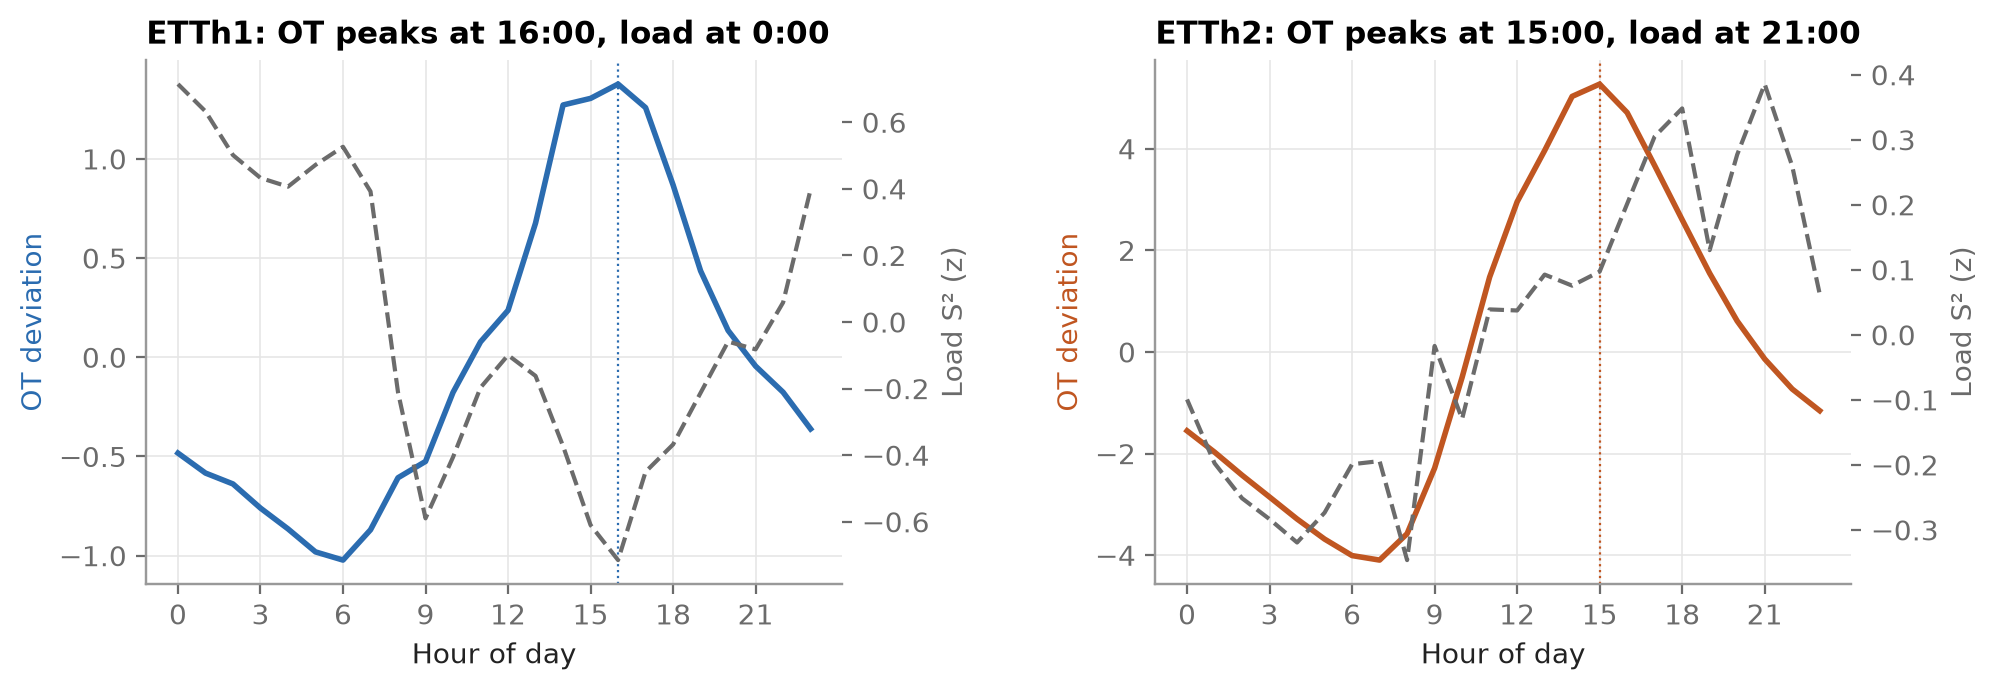
\includegraphics[width=\textwidth,height=3.9cm,keepaspectratio]{eda_daily_profile}
  \vspace{0.1cm}
  \begin{columns}[T]
    \begin{column}{0.49\textwidth}\scriptsize
      \begin{itemize}
        \item Oil temperature and load correlate weakly (r$\approx$0.22, deseasonalised)
        \item Load acts \hl{with a delay}: ETTh1 tracks load smoothed at an 18 h half-life (large thermal mass)
      \end{itemize}
    \end{column}
    \begin{column}{0.49\textwidth}\scriptsize
      \begin{itemize}
        \item \hl{Missing ambient temperature is the data's biggest limit}; models can only proxy it with hour/season cycles
        \item Design: heating $\propto$ current² (S² = useful² + useless²), smoothed at several time constants (IEC 60076-7)
      \end{itemize}
    \end{column}
  \end{columns}
  \source{Seasonal component removed with a centred 30-day moving average (descriptive only; not used by the models).}
\end{frame}

% ------------------------------------------------------------------ 5 inertia & drift
\settag{EDA ③ Inertia and year-to-year change}
\begin{frame}{Persistence suffices 1 h ahead, but ETTh1 runs 7.7 °C cooler in the evaluation year, so models must be robust across years}
  \begin{columns}[T]
    \begin{column}{0.60\textwidth}
      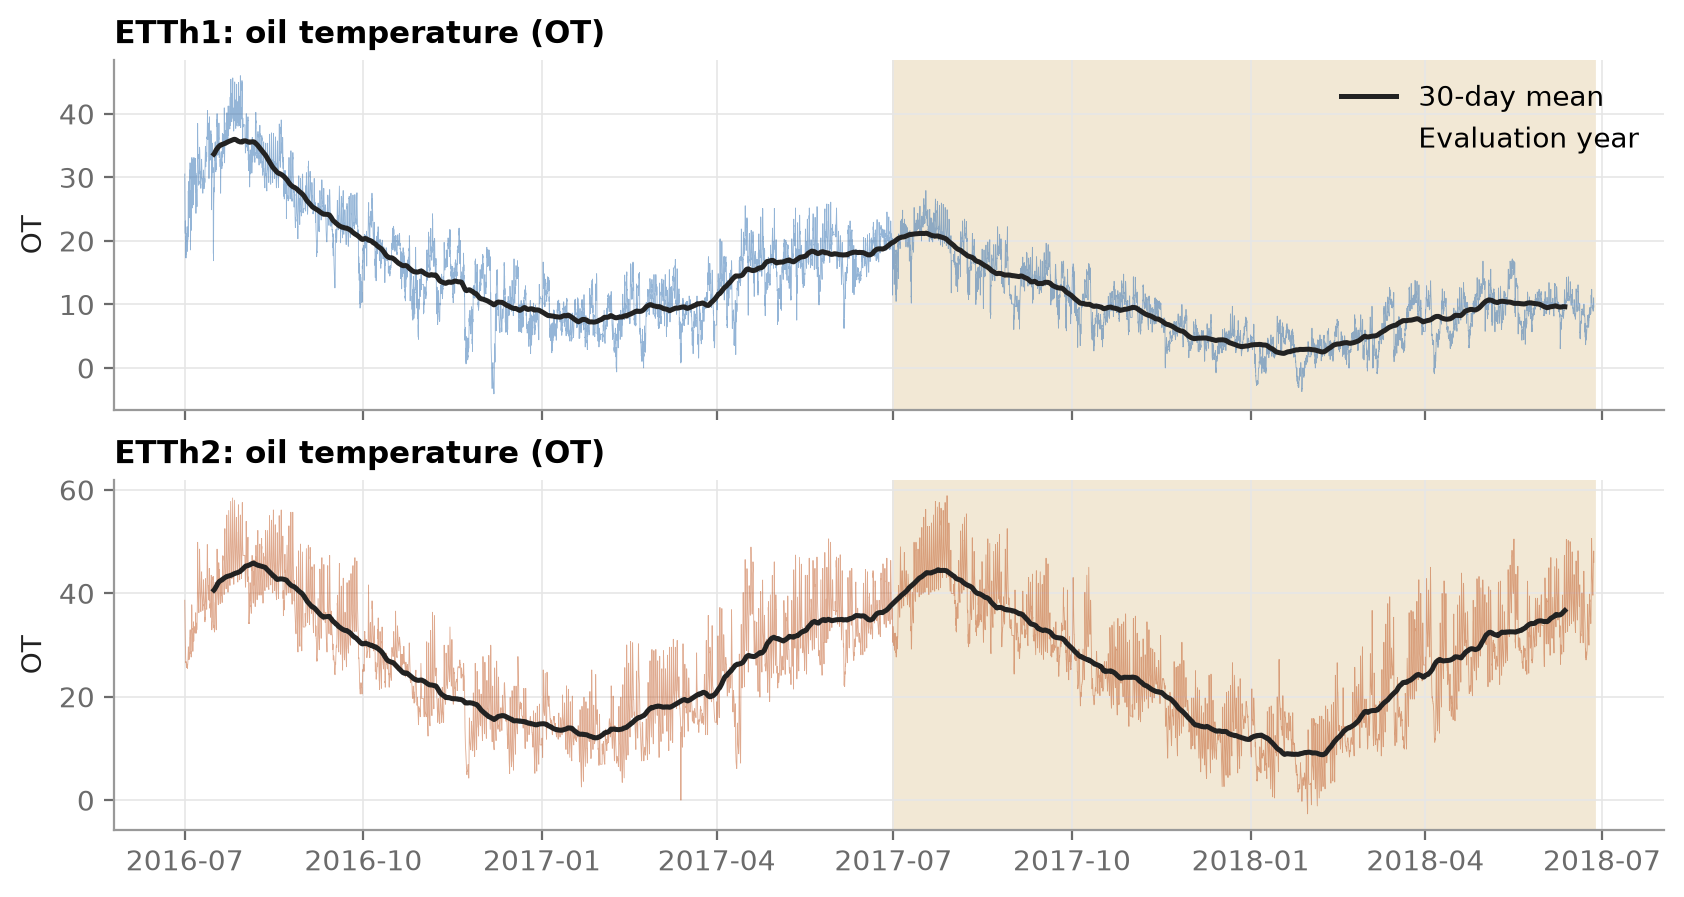
\includegraphics[width=\textwidth,height=4.0cm,keepaspectratio]{eda_ot_overview}
    \end{column}
    \begin{column}{0.38\textwidth}
      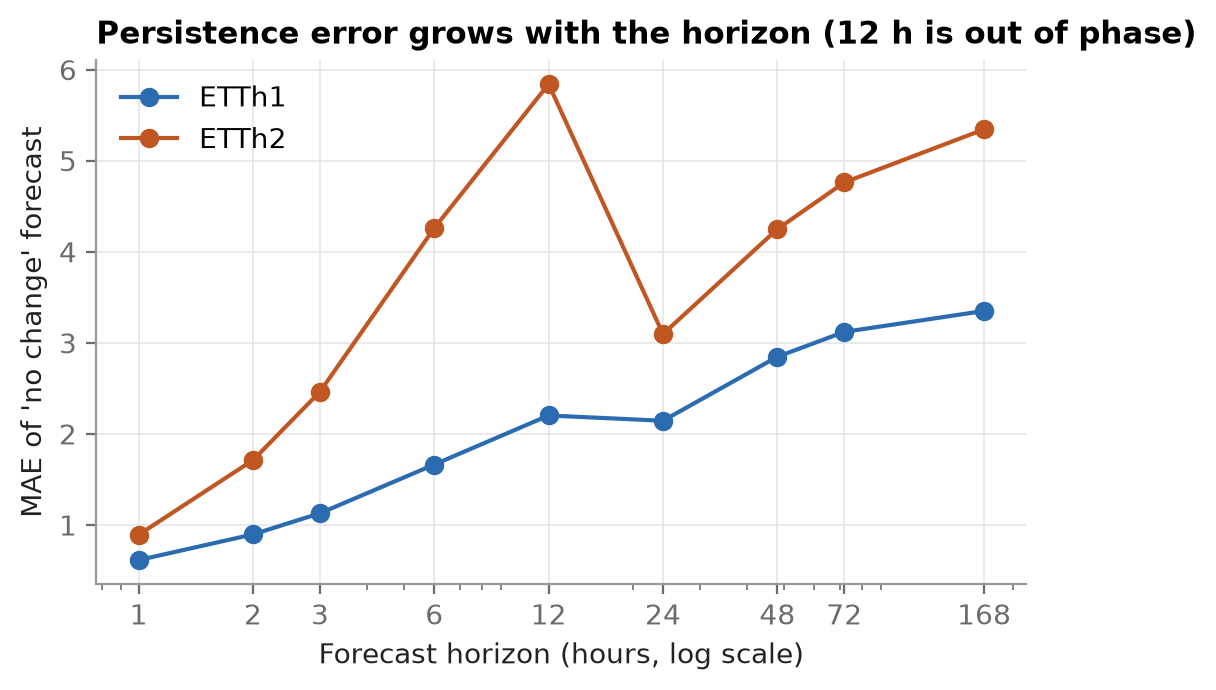
\includegraphics[width=\textwidth,height=4.0cm,keepaspectratio]{eda_persistence_horizon}
    \end{column}
  \end{columns}
  \vspace{0.05cm}
  \scriptsize
  \begin{itemize}\setlength{\itemsep}{1pt}
    \item 24 h autocorrelation 0.94; persistence error 0.6 °C at 1 h, 2.1 °C at 24 h (ETTh1). \hl{Value lies hours to a day ahead}
    \item ETTh1's evaluation year is 7.7 °C cooler, peaking at 27.9 °C, below the proxy alarm (35.2 °C). \hlb{Models that cannot extrapolate degrade}
  \end{itemize}
\end{frame}

% ------------------------------------------------------------------ 6 approach
\settag{Approach and design decisions}
\begin{frame}{From the EDA we chose a simple, robust design: physics features, forecasting the temperature change, rolling validation}
  \scriptsize
  \renewcommand{\arraystretch}{1.25}
  \begin{tabularx}{\textwidth}{>{\bfseries}p{3.0cm} X X}
    \toprule
    Decision & What & Why \\
    \midrule
    Forecast the change & Learn OT(T)−OT(t) and add it to the current value & Level shifts between years (p.6); trees cannot extrapolate outside the training range \\
    Physics features & S² ($\propto$ current²), smoothing at 3/12/48 h, thermal time-constant estimate & IEC 60076-7 first-order thermal model; delayed load effect (p.5) \\
    Strong benchmark & Skill vs. persistence and the Diebold--Mariano test & Naive forecasts are strong for slowly changing series (Cui et al. 2021, Hewamalage et al. 2023) \\
    Rolling validation & Refit monthly over 12 months, covering all seasons; tuning on development data only & A single spring test split gives season-dependent conclusions \\
    Data-quality handling & Detect stuck sensors and spikes from past data only; fall back to persistence & The defects of p.4 can occur in operation too \\
    Interval calibration & Quantile regression + conformal calibration (CQR) & Interval under-coverage is a known issue (Tembo et al. 2025) \\
    \bottomrule
  \end{tabularx}
  \source{Models: grey-box physics, Ridge, GBM (3 variants), physics + GBM hybrid, MLP, raw-window linear (DLinear-style), LSTM, ensemble. See appendix.}
\end{frame}

% ------------------------------------------------------------------ 7 protocol
\settag{Evaluation protocol}
\begin{frame}{The evaluation never looks into the future and measures generalisation across all seasons with 12 monthly rolling folds}
  \centering
  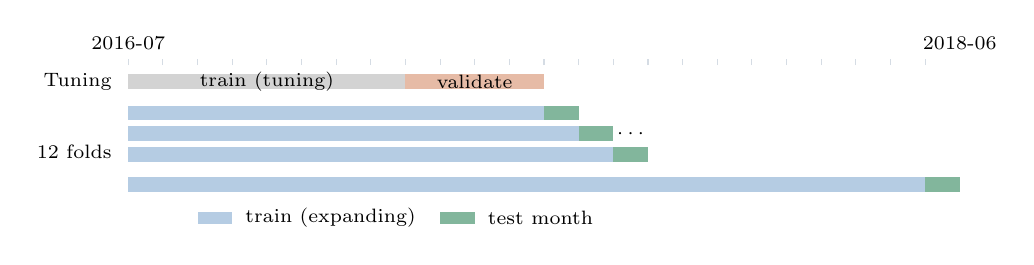
\begin{tikzpicture}[x=0.44cm,y=0.38cm,font=\scriptsize]
    \foreach \i in {0,...,23} { \draw[rule] (\i,0.6) -- (\i,0.8); }
    \node[above] at (0,0.8) {2016-07};
    \node[above] at (24,0.8) {2018-06};
    \fill[muted!30] (0,-0.2) rectangle (8,0.3); \node at (4,0.05) {train (tuning)};
    \fill[accent2!40] (8,-0.2) rectangle (12,0.3); \node at (10,0.05) {validate};
    \node[left] at (-0.2,0.05) {Tuning};
    \foreach \k/\y in {0/-1.0,1/-1.7,2/-2.4} {
      \fill[accent!35] (0,\y-0.25) rectangle (12+\k,\y+0.25);
      \fill[good!60] (12+\k,\y-0.25) rectangle (13+\k,\y+0.25);
    }
    \node at (14.5,-1.7) {$\cdots$};
    \fill[accent!35] (0,-3.65) rectangle (23,-3.15); \fill[good!60] (23,-3.65) rectangle (24,-3.15);
    \node[left] at (-0.2,-2.3) {12 folds};
    \fill[accent!35] (2,-4.7) rectangle (3,-4.3); \node[right] at (3.1,-4.5) {train (expanding)};
    \fill[good!60] (9,-4.7) rectangle (10,-4.3); \node[right] at (10.1,-4.5) {test month};
  \end{tikzpicture}
  \vspace{0.1cm}
  \begin{columns}[T]
    \begin{column}{0.32\textwidth}\footnotesize
      \textbf{No leakage}
      \begin{itemize}
        \item Each month refitted at its first issue time with labels known then
        \item Thresholds and calibration: development data only
      \end{itemize}
    \end{column}
    \begin{column}{0.32\textwidth}\footnotesize
      \textbf{Metrics}
      \begin{itemize}
        \item MAE, RMSE, skill vs. persistence
        \item No MAPE: OT nears 0 °C
      \end{itemize}
    \end{column}
    \begin{column}{0.32\textwidth}\footnotesize
      \textbf{Significance}
      \begin{itemize}
        \item Diebold--Mariano test, HAC variance for overlapping 24 h forecasts
        \item Holm correction across the 24 comparisons
      \end{itemize}
    \end{column}
  \end{columns}
  \source{References: Tashman (2000), Hewamalage, Ackermann \& Bergmeir (2023), Diebold \& Mariano (1995), Harvey et al. (1997)}
\end{frame}

% ------------------------------------------------------------------ 8 accuracy
\settag{Results ① Accuracy}
\begin{frame}{The linear model with the plan cuts 24 h error by 9.1\% (ETTh1) and 4.8\% (ETTh2); the ensemble narrowly leads on ETTh2}
  \centering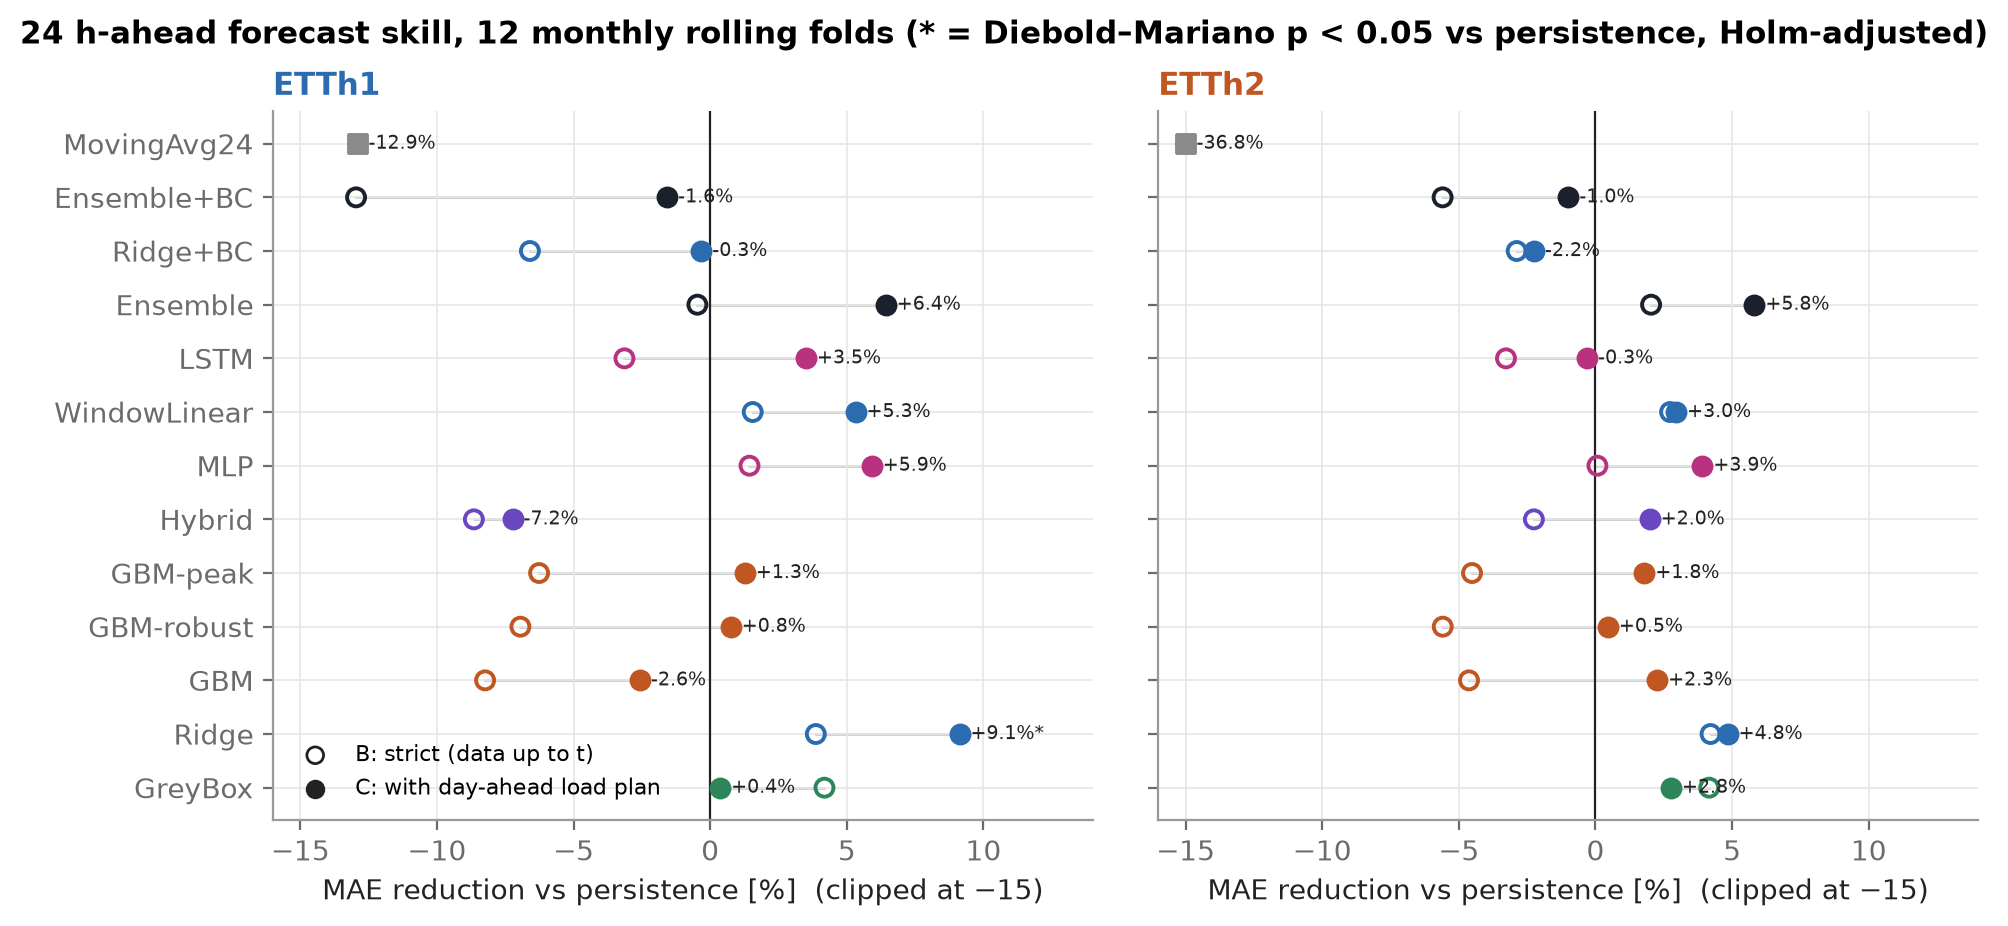
\includegraphics[width=\textwidth,height=3.9cm,keepaspectratio]{res_skill}\par\raggedright
  \scriptsize
  \begin{itemize}\setlength{\itemsep}{1pt}
    \item MAE: ETTh1 1.76 → \hl{1.60 °C} (Holm-adjusted p<0.001), ETTh2 3.25 → \hl{3.09 °C} (p=0.004 unadjusted; 0.10 after Holm, so not significant)
    \item \hl{The plan (C)} helps every model except the physics model alone (ETTh1 Ridge 3.9\% → 9.1\%), which gets worse on both stations: the benefit is model-dependent
  \end{itemize}
\end{frame}

% ------------------------------------------------------------------ 9 complexity
\settag{Results ② Model complexity}
\begin{frame}{More complex is not better: GBM, LSTM and MLP did not beat the linear model under year-to-year drift}
  \scriptsize
  \renewcommand{\arraystretch}{1.08}
  \begin{tabularx}{\textwidth}{>{\bfseries}p{4.2cm} c c X}
    \toprule
    Method (C: with plan) & ETTh1 & ETTh2 & Interpretation \\
    \midrule
    Ridge (physics features) & \hlg{+9.1\%*} & +4.8\% & Best on ETTh1. Few parameters, extrapolates well \\
    Ensemble (Ridge+GBM+Hybrid) & +6.4\% & \hlg{+5.8\%} & Best on ETTh2, 1 point ahead of Ridge \\
    MLP (64-32) & +5.9\% & +3.9\% & Short of the linear model \\
    Raw-window linear (DLinear-style) & +5.3\% & +2.9\% & Competitive without feature design (consistent with Zeng et al. 2023) \\
    LSTM (raw sequence) & +3.5\% & −0.3\% & No clear advantage for sequence models \\
    GBM / robust GBM / peak GBM & −2.6 to +1.3\% & +0.5 to +2.3\% & −4 to −8\% without the plan (B); weak under level shifts \\
    Physics + GBM hybrid & −7.2\% & +2.0\% & Fails to learn the physics model's residual \\
    Bias correction from past 7 days (+BC) & worse & worse & Errors are weather-driven swings, not persistent bias \\
    \bottomrule
  \end{tabularx}
  \vspace{0.15cm}
  \softbox{}{\scriptsize\textbf{Implication}: accuracy seems limited by \hl{input information (no ambient temperature)} more than model capacity. Prioritise data over complexity (a hypothesis to test with ambient data).}
  \source{Figures are the reduction in 24 h MAE vs. persistence. * = Diebold--Mariano p<0.05 after Holm correction across each station's comparisons.}
\end{frame}

% ------------------------------------------------------------------ 10 horizons
\settag{Results ③ Forecast lead time}
\begin{frame}{Forecasts help most hours to half a day ahead (up to 22--53\% lower error) and only 5--9\% at 24 h, so match the horizon to the use}
  \centering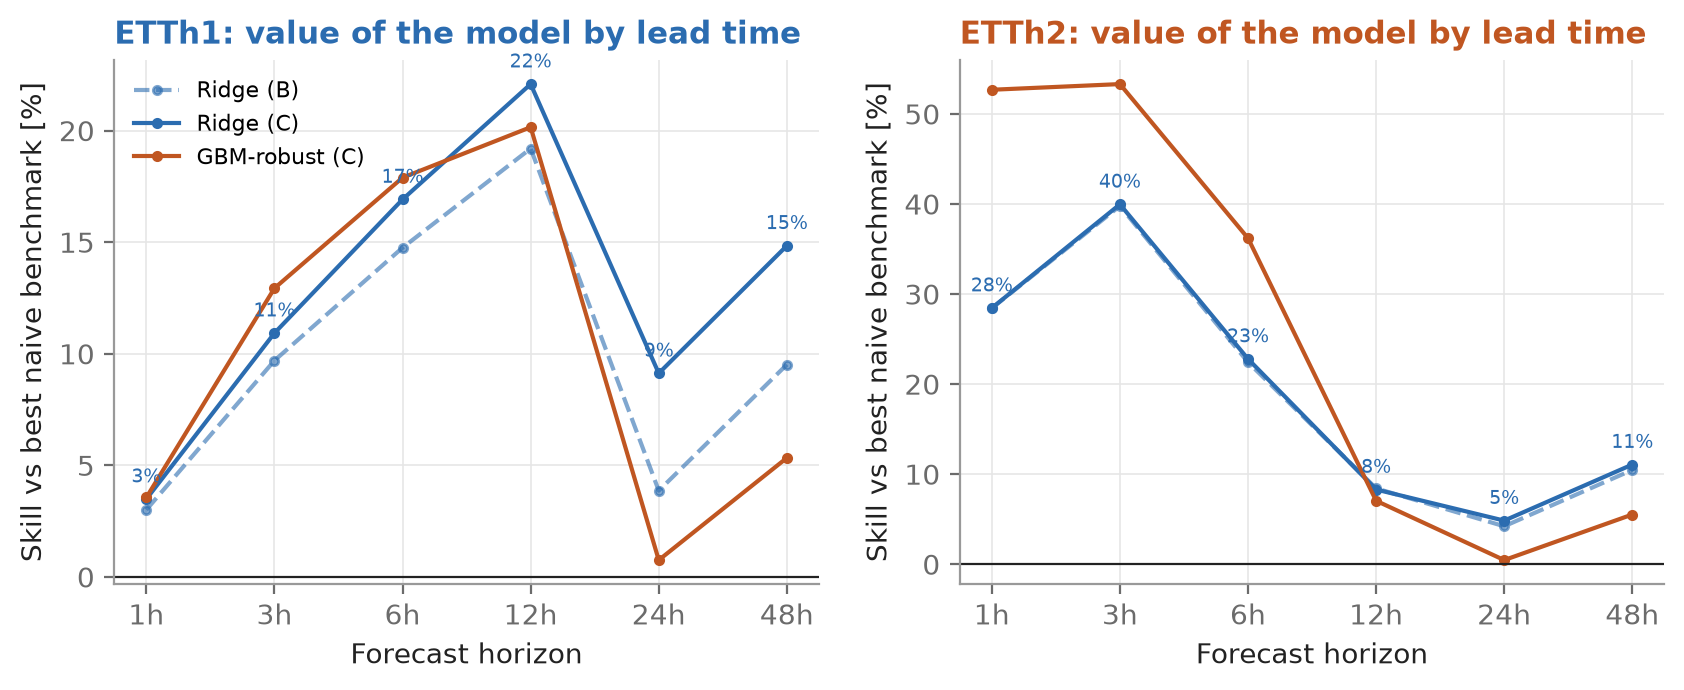
\includegraphics[width=\textwidth,height=3.7cm,keepaspectratio]{res_horizons}\par\raggedright
  \scriptsize
  \begin{itemize}\setlength{\itemsep}{1pt}
    \item \textbf{1--6 h}: robust GBM best; ETTh2 error −53\% at 1 h and 3 h, −36\% at 6 h (learns the daily heating pattern)
    \item \textbf{12--48 h}: linear with plan (C) best; ETTh1 −22\% at 12 h. ETTh2 at 12 h only −8\% (``same hour yesterday'' is strong)
    \item \hl{Use}: $\leq$6 h for load and cooling decisions, 24 h for inspection and maintenance planning (alerts: p.12)
  \end{itemize}
  \source{Benchmark: better of persistence and ``same hour yesterday''; same 12 rolling folds.}
\end{frame}

% ------------------------------------------------------------------ 11 alerts
\settag{Business value ① Early overheating warning}
\begin{frame}{With a 4 °C warning margin, 80\% of overheating onsets are flagged about 23 h ahead, with false alerts held to about 10 h per month}
  \begin{columns}[T]
    \begin{column}{0.50\textwidth}
      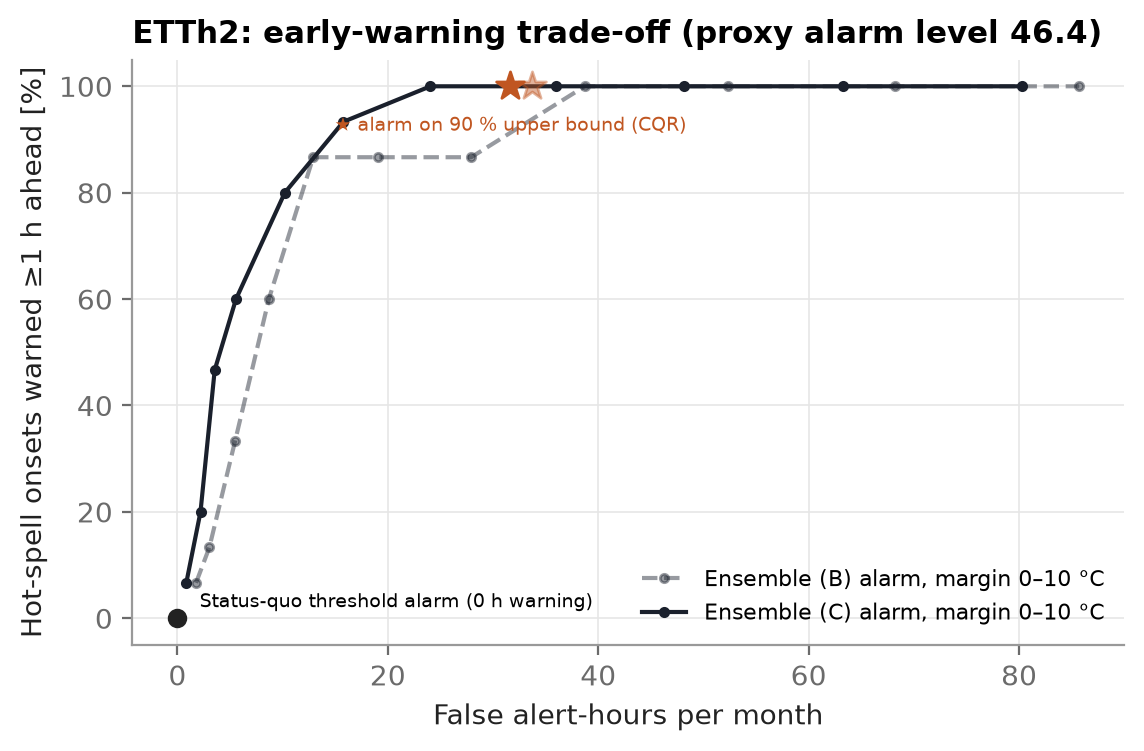
\includegraphics[width=\textwidth]{res_alert_tradeoff}
    \end{column}
    \begin{column}{0.48\textwidth}
      \scriptsize
      \renewcommand{\arraystretch}{1.2}
      \begin{tabular}{l c c}
        \toprule
        Alert rule & Warned & False h/mo \\
        \midrule
        Today: threshold & 0\% & -- \\
        Forecast (B) + 4 °C & 87\% & 12.9 \\
        \textbf{Forecast (C) + 4 °C} & \hlg{80\%} & \hlg{10.2} \\
        Forecast (C) + 5 °C & 93\% & 15.8 \\
        90\% interval upper bound & 100\% & 31.6 \\
        \bottomrule
      \end{tabular}
      \vspace{0.1cm}
      \begin{itemize}\setlength{\itemsep}{1pt}
        \item The margin is \hl{the operator's dial}: false-alarm vs. miss cost
        \item 4 °C was \hl{read off the evaluation curve}; fix it in the shadow run
        \item For alerts the plan adds little
        \item ETTh1 never reaches the proxy alarm; not scored
      \end{itemize}
    \end{column}
  \end{columns}
  \source{ETTh2, ensemble. Onset: proxy alarm (46.4 °C) crossed after $\geq$24 h below; 15 onsets. 13 of 620 alerts unscorable (missing truth).}
\end{frame}

% ------------------------------------------------------------------ 12 uncertainty
\settag{Business value ② Communicating uncertainty}
\begin{frame}{The quantile-regression ``90\% interval'' actually covered only 75--84\%, but conformal calibration brought it to 90\%}
  \begin{columns}[T]
    \begin{column}{0.62\textwidth}
      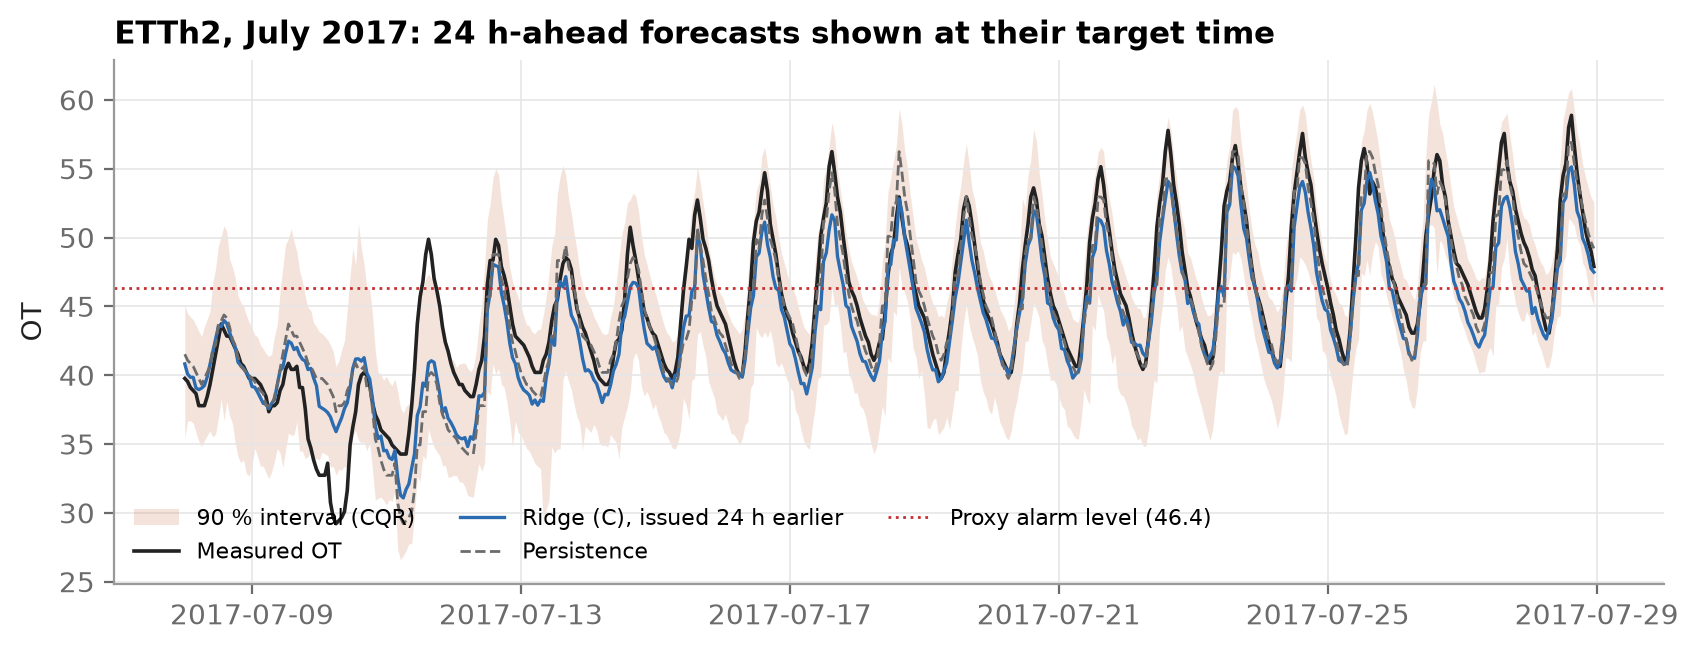
\includegraphics[width=\textwidth]{res_example_forecast}
    \end{column}
    \begin{column}{0.36\textwidth}
      \scriptsize
      \renewcommand{\arraystretch}{1.25}
      \begin{tabular}{l c c}
        \toprule
        & Raw & \textbf{After CQR} \\
        \midrule
        Coverage ETTh1 & 84\% & \hlg{90\%} \\
        Coverage ETTh2 & 75\% & \hlg{91\%} \\
        Width ETTh1 & 6.0 °C & 7.3 °C \\
        Width ETTh2 & 9.0 °C & 13.0 °C \\
        \bottomrule
      \end{tabular}
      \vspace{0.2cm}
      \begin{itemize}\setlength{\itemsep}{2pt}
        \item \hl{Check stated confidence on real data} before maintenance use
        \item Width (ETTh2 about ±6.5 °C) likely reflects the missing ambient temperature
      \end{itemize}
    \end{column}
  \end{columns}
  \source{CQR: Romano et al. (2019); last 60 days before each refit calibrate. Framing C. Coverage is measured, not guaranteed; fallback hours excluded.}
\end{frame}

% ------------------------------------------------------------------ 13 robustness
\settag{Business value ③ Load-plan quality requirement}
\begin{frame}{The plan's benefit fades at 5--10\% plan error and at 20\% both stations fall below the no-plan forecast: plan accuracy is a precondition}
  \begin{columns}[T]
    \begin{column}{0.55\textwidth}
      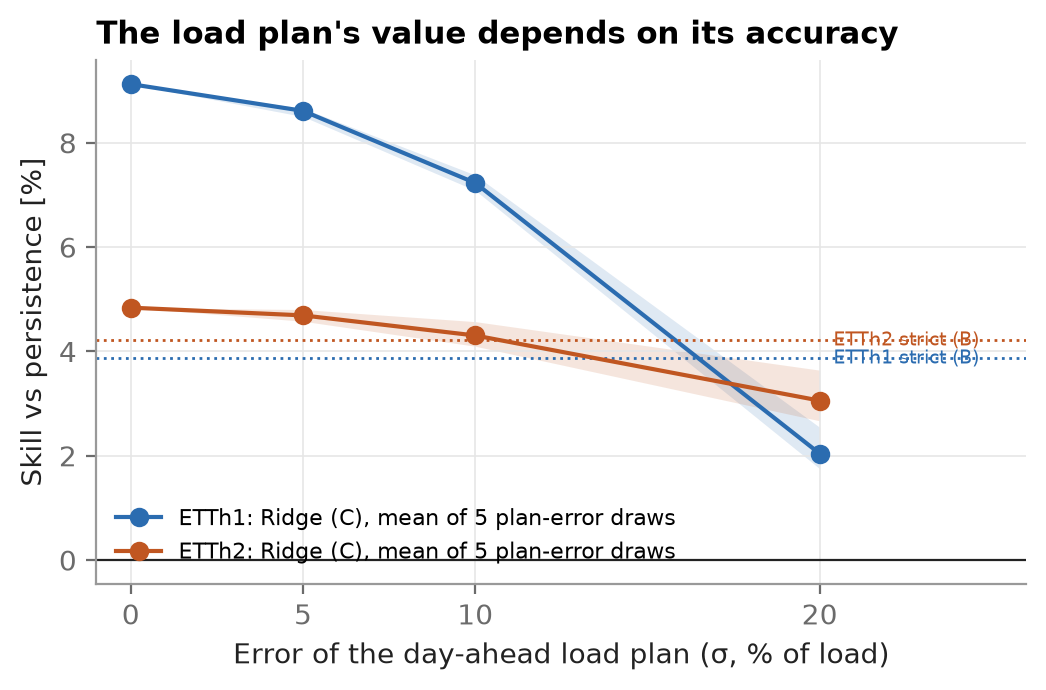
\includegraphics[width=\textwidth]{res_load_noise}
    \end{column}
    \begin{column}{0.43\textwidth}
      \footnotesize
      \begin{itemize}\setlength{\itemsep}{3pt}
        \item ``Imperfect plan'': daily bias + hourly noise (σ) added to future load only; mean of 5 draws
        \item ETTh1: skill 9.1\% (no error) → 7.2\% (10\%) → \hlb{2.0\% (20\%)}, below no plan (3.9\%)
        \item ETTh2: 4.8\% → 4.3\% (10\%, ≈ no plan 4.2\%) → \hlb{3.1\% (20\%)}
        \item \hl{Requirement}: plan error within about 5--10\%; otherwise use B
      \end{itemize}
    \end{column}
  \end{columns}
  \source{Trained on true load; plan error added only at evaluation, never to measured history. Band: min--max of 5 draws. Model: Ridge (C).}
\end{frame}

% ------------------------------------------------------------------ 14 failure analysis
\settag{Error analysis}
\begin{frame}{Errors concentrate at season changes and in hot periods; in ETTh2's hottest range the models do worse than persistence}
  \centering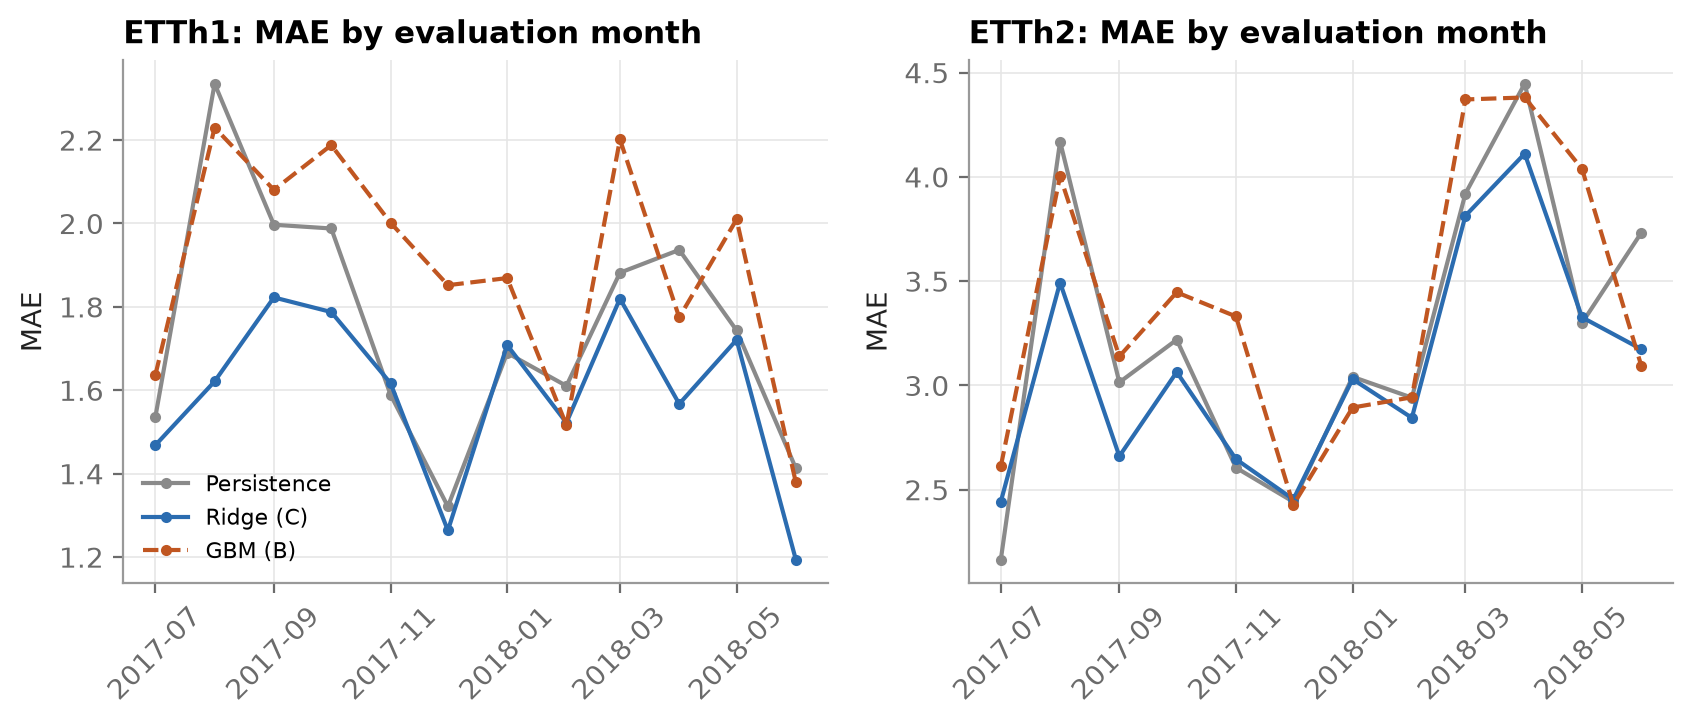
\includegraphics[width=\textwidth,height=3.6cm,keepaspectratio]{res_monthly}\par\raggedright
  \scriptsize
  \begin{itemize}\setlength{\itemsep}{1pt}
    \item Hot-period MAE (above the development 90th pct., ETTh2): persistence \textbf{2.69 °C}, Ridge (C) 3.04, peak GBM 3.07. \hlb{Models pull peaks to the mean}
    \item No model beats it; closest are LSTM (C) 2.76 °C and MLP (C) 2.79 °C. A hot-range model or ambient temperature could help
    \item The alert margin offsets this under-prediction (p.12)
  \end{itemize}
\end{frame}

% ------------------------------------------------------------------ 15 anomaly
\settag{Extension ① Anomaly detection}
\begin{frame}{Data-quality monitoring can start now, but detecting cooling faults from the expected-temperature gap needs ambient temperature}
  \begin{columns}[T]
    \begin{column}{0.49\textwidth}
      \softbox{}{\footnotesize\textbf{Rule-based data-quality monitoring: works}
      \begin{itemize}\setlength{\itemsep}{1pt}
        \item Detects stuck load sensors, OT spikes and all-channel freezes from past data (after 24 h / 12 h of constancy). Load balance is descriptive only
        \item Found a real \hl{43-day stuck sensor} (p.4)
        \item A stuck load sensor switches forecasts to persistence (continuity, not necessarily conservative)
      \end{itemize}}
    \end{column}
    \begin{column}{0.49\textwidth}
      \softbox{}{\footnotesize\textbf{Residual-based cooling-fault detection: not yet}
      \begin{itemize}\setlength{\itemsep}{1pt}
        \item Alarm on the 6 h mean gap to load-based expected OT (Djamali \& Tenbohlen; CIGRE digital twin)
        \item +3--8 °C synthetic faults caught \hlb{0\%} (0 of 180): the model ``follows'' the fault, so the gap stays below the threshold (1.5--1.7 °C)
        \item +20 °C in 12 h: all caught on ETTh1 (ETTh2: 10\%)
      \end{itemize}}
    \end{column}
  \end{columns}
  \vspace{0.2cm}
  \footnotesize
  \textbf{Conclusion}: re-test fault detection with ambient temperature and cooling status as inputs; for now deploy data-quality monitoring only.
  \source{Synthetic fault: 12 h rise, held 36 h; 30 per size at the same onsets, only where the unmodified data are clean and alarm-free.}
\end{frame}

% ------------------------------------------------------------------ 16 limitations
\settag{Current limitations}
\begin{frame}{This PoC shows promise on public data only; real-asset value needs ambient temperature, alarm levels and fault history}
  \scriptsize
  \renewcommand{\arraystretch}{1.3}
  \begin{tabularx}{\textwidth}{>{\bfseries}p{3.4cm} X X}
    \toprule
    Limitation & Impact & What resolves it \\
    \midrule
    No ambient temperature & The likely daily-cycle driver is missing; probably limits accuracy and fault detection & Hourly temperature, nearest weather station \\
    No alarm levels or fault history & Proxy alarm only; avoided loss cannot be costed & Alarm settings, maintenance records \\
    Few evaluation events & 15 onsets only; uncertain warning rates & More transformers and periods \\
    Only two transformers & Generalisation untested; the two differ widely & Asset register, multi-unit data \\
    Load plan simulated & Real plan accuracy and timing unknown & Actual day-ahead plans \\
    \bottomrule
  \end{tabularx}
\end{frame}

% ------------------------------------------------------------------ 17 next steps
\settag{Next steps}
\begin{frame}{We propose adding ambient temperature and a 3-month shadow run, then deploying forecast alerts once acceptance criteria are met}
  \centering
  \begin{tikzpicture}[font=\scriptsize, node distance=0.35cm,
      stepbox/.style={draw=accent, thick, fill=soft, rounded corners=2pt, text width=3.95cm, minimum height=2.9cm, align=left, inner sep=5pt}]
    \node[stepbox] (a) {\textbf{\color{accent}Step 1 (1 month)\\Enrich the data}\\[3pt]
      ・Connect ambient temperature\\・Share alarm levels, maintenance records\\・Start data-quality monitoring\\[3pt]
      \textbf{Proposed pass}: ambient temperature improves MAE by $\geq$10\%};
    \node[stepbox, right=of a] (b) {\textbf{\color{accent}Step 2 (3 months)\\Shadow run}\\[3pt]
      ・Show forecasts beside operations (not for decisions)\\・Log false alerts and misses\\[3pt]
      \textbf{Proposed pass}: $\geq$80\% warned $\geq$12 h ahead, $\leq$10 false alert-hours/month};
    \node[stepbox, right=of b] (c) {\textbf{\color{accent}Step 3\\Deploy and scale}\\[3pt]
      ・Add alerts to maintenance procedures\\・Re-test cooling-fault detection\\・Extend to more transformers\\[3pt]
      \textbf{Monitor}: monthly coverage, error, drift; retrain};
    \draw[->,thick,accent] (a) -- (b);
    \draw[->,thick,accent] (b) -- (c);
  \end{tikzpicture}
  \vspace{0.3cm}
  \footnotesize
  \begin{itemize}
    \item This PoC's code (data-quality checks, features, rolling validation, interval calibration, alert simulation) can be reused as the Step 2 evaluation platform; features are computed without labels (connection to live systems not built)
  \end{itemize}
\end{frame}

% ------------------------------------------------------------------ appendix
\settag{Appendix A  Models compared}
\begin{frame}{Appendix: models compared and their settings}
  \scriptsize
  \renewcommand{\arraystretch}{1.2}
  \begin{tabularx}{\textwidth}{>{\bfseries}p{3.2cm} X}
    \toprule
    Model & Description \\
    \midrule
    Persistence / 24 h moving avg. & Benchmarks. At 24 h, persistence equals ``same hour yesterday'' \\
    Grey-box thermal model & Discretised IEC 60076-7 first-order model. Learns time constant τ (estimated 36--48 h) and load gain. Ambient proxied by season/hour harmonics and weekly mean oil temperature \\
    Ridge & Physics features (S², S² exponential smoothing at 3/12/48 h, oil-temperature change, calendar). Regularisation chosen on development data \\
    GBM / robust / peak & HistGradientBoosting. Robust: drops the oil-temperature level and up-weights recent data (half-life 180 days). Peak: top 10\% weighted ×3 \\
    Hybrid & GBM trained on the grey-box residual \\
    MLP / LSTM & MLP (64-32). LSTM: raw past 72 h + (C) next 24 h of plan. Both early-stop on the chronologically last part of the training data \\
    Raw-window linear & Ridge on past 168 h of oil temperature and S² (+24 h of plan) (DLinear-style) \\
    Ensemble / +BC & Equal-weight mean of Ridge, robust GBM and hybrid. +BC: subtract the mean error of the past 7 days \\
    CQR & Quantile GBM (5\%, 95\%) + conformal calibration \\
    \bottomrule
  \end{tabularx}
\end{frame}

\settag{Appendix B  References}
\begin{frame}{Appendix: references}
  \tiny
  \begin{enumerate}\setlength{\itemsep}{0pt}
    \item H. Zhou et al. Informer: Beyond Efficient Transformer for Long Sequence Time-Series Forecasting. AAAI 2021. (ETT dataset, CC BY-ND 4.0)
    \item IEC 60076-7:2018 Loading guide for mineral-oil-immersed power transformers. / IEEE Std C57.91-2011.
    \item F. Tembo et al. Data-Driven vs Traditional Approaches to Power Transformer's Top-Oil Temperature Estimation. arXiv:2501.16831, 2025.
    \item M. Djamali, S. Tenbohlen. Malfunction Detection of the Cooling System in Air-Forced Power Transformers Using Online Thermal Monitoring. IEEE Trans. Power Delivery, 2017.
    \item CIGRE Technical Brochure 995. Digital twins for power transformers: concept and future perspectives. 2026.
    \item H. Hewamalage, K. Ackermann, C. Bergmeir. Forecast evaluation for data scientists: common pitfalls and best practices. Data Min. Knowl. Disc. 37, 2023.
    \item Y. Cui, J. Xie, K. Zheng. Historical Inertia: A Neglected but Powerful Baseline for Long Sequence Time-Series Forecasting. CIKM 2021.
    \item A. Zeng et al. Are Transformers Effective for Time Series Forecasting? AAAI 2023.
    \item F. X. Diebold, R. S. Mariano. Comparing Predictive Accuracy. JBES, 1995. / D. Harvey, S. Leybourne, P. Newbold. IJF, 1997.
    \item L. Tashman. Out-of-sample tests of forecasting accuracy. IJF, 2000.
    \item T. Januschowski et al. Forecasting with trees. IJF, 2022.
    \item J. Smith, K. F. Wallis. A Simple Explanation of the Forecast Combination Puzzle. Oxford Bull. Econ. Stat., 2009.
    \item Y. Romano, E. Patterson, E. Candès. Conformalized Quantile Regression. NeurIPS 2019.
  \end{enumerate}
  \vspace{0.2cm}
  {\scriptsize\color{muted}Code and full results: GitHub repository (reproduction steps in the README)}
\end{frame}

\end{document}
